%%%%%%%%%%%%%%%%%%%%%%%%%%%%%%%%%%%%%%%%%
% Beamer Presentation
% LaTeX Template
% Version 1.0 (10/11/12)
%
% This template has been downloaded from:
% http://www.LaTeXTemplates.com
%
% License:
% CC BY-NC-SA 3.0 (http://creativecommons.org/licenses/by-nc-sa/3.0/)
%
%%%%%%%%%%%%%%%%%%%%%%%%%%%%%%%%%%%%%%%%%

\documentclass{beamer}

\mode<presentation> {
\usetheme{Madrid}
}

\usepackage[utf8]{inputenc}
\usepackage[spanish]{babel}
\usepackage{graphicx}
\usepackage{booktabs}
\usepackage{xcolor}

\title[Introducción a Git]{Introducción a Git}

\author{Rubén Crespo Cano}
\institute[]
{
{\color{gray}\textit{@rcrespocano}}
}
\date{}

\begin{document}

\begin{frame}
\titlepage
\end{frame}

\begin{frame}
\frametitle{¿Qué es git?}
\begin{itemize}
\item Sistema de control de versiones (VCS)
\item Sistema distribuido
\item Creado por Linus Torvalds para Linux (2005)
\item Interfaz de línea de comandos (aunque también existen interfaces gráficas)
\end{itemize}
\vskip 0.25cm
\begin{figure}

\includegraphics[width=0.50\linewidth]{img/gitlogo.png}
\end{figure}
\end{frame}

\begin{frame}
\frametitle{Sobre control de versiones}
Un sistema de control de versiones registra y almacena cambios en ficheros a lo largo del tiempo para mejorar la gestión y poder recuperar versiones específicas en cualquier momento.
\vskip 0.50cm
\begin{itemize}
\item Sistema de control de versiones local
\item Sistema de control de versiones centralizado
\item Sistema de control de versiones distribuido
\end{itemize}
\end{frame}

\begin{frame}
\frametitle{Sistema de control de versiones local}
\begin{figure}
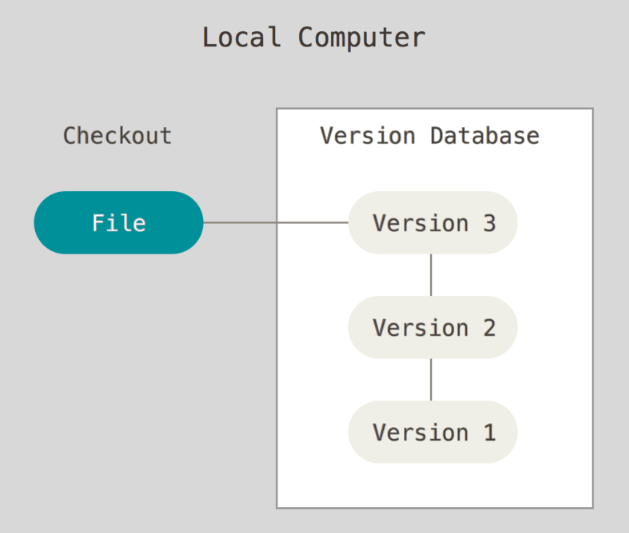
\includegraphics[width=0.50\linewidth]{img/local.png}
\end{figure}
\end{frame}

\begin{frame}
\frametitle{Sistema de control de versiones centralizado}
\begin{figure}
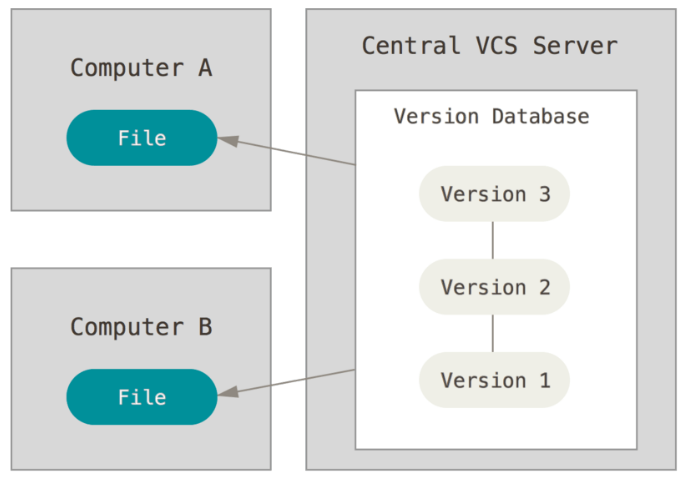
\includegraphics[width=0.50\linewidth]{img/centralized.png}
\end{figure}
\end{frame}

\begin{frame}
\frametitle{Sistema de control de versiones centralizado}
\begin{itemize}
\item Un servidor centralizado contiene todos los ficheros versionados y los metadatos.
\item Ventajas: colaboración, administración y sencillez
\item Inconvenientes: centralización, disponibilidad, copias de seguridad, velocidad, etc.
\end{itemize}
\end{frame}

\begin{frame}
\frametitle{Sistema de control de versiones distribuido}
\begin{figure}
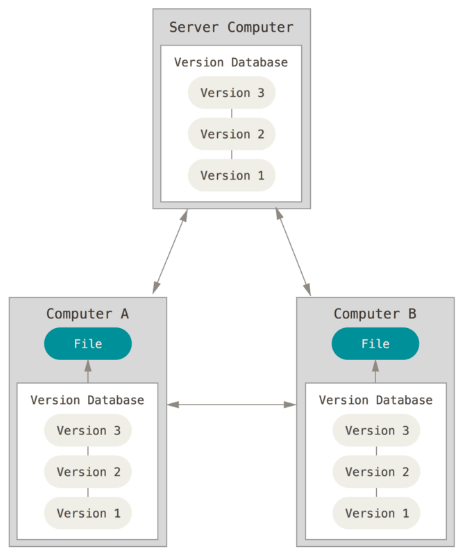
\includegraphics[width=0.50\linewidth]{img/distributed.png}
\end{figure}
\end{frame}

\begin{frame}
\frametitle{Sistema de control de versiones distribuido}
\begin{itemize}
\item Cada cliente tiene una réplica exacta del repositorio (ficheros, metadatos, historial, etc.)
\item Si el servidor muere cualquier copia puede reemplazar al servidor central
\item Colaboración con distintos grupos de forma descentralizada
\item Ventajas
\begin{itemize}
\item Velocidad
\item Diseño simple
\item Soporte para desarrollo no lineal (cientos de ramas paralelas)
\item Totalmente distribuido
\item Capaz de gestionar grandes proyectos de forma eficiente (velocidad y tamaño de datos)
\end{itemize}
\item Inconvenientes: curva aprendizaje
\end{itemize}
\end{frame}

\begin{frame}
\frametitle{¿Quién utiliza git?}
\begin{figure}

\includegraphics[width=0.95\linewidth]{img/who.png}
\end{figure}
\vskip 0.5cm
\small
Microsoft, Amazon, LinkedIn, Cisco, IBM, Accenture, Facebook, Yahoo, Apple, T-Mobile, Lenovo, Atlassian, y muchas otras.
\small
\begin{itemize}
\item https://git-scm.com/
\item https://www.quora.com/What-companies-use-Git
\end{itemize}
\end{frame}

\begin{frame}
\frametitle{Flujo de trabajo}
\begin{figure}
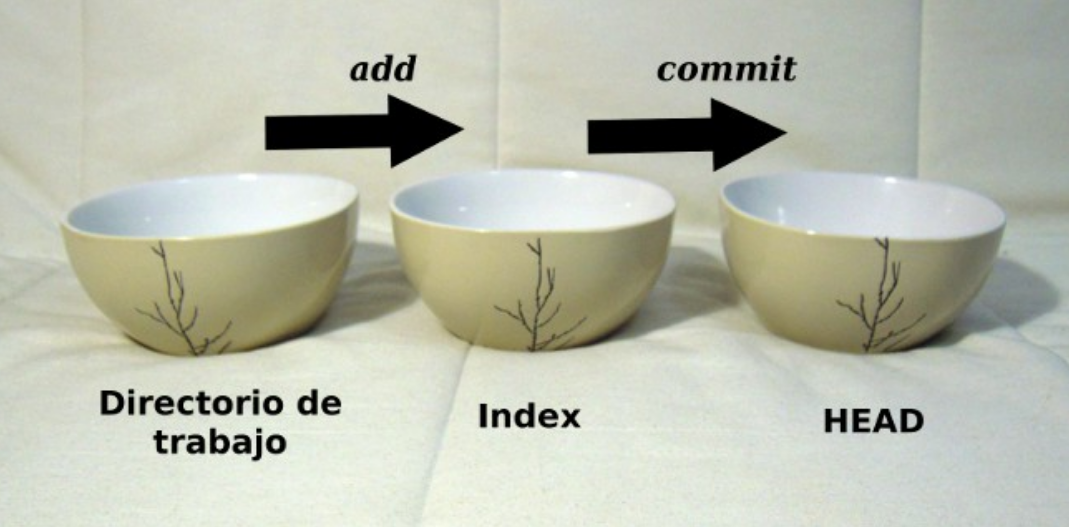
\includegraphics[width=0.8\linewidth]{img/cuencos.png}
\end{figure}
\end{frame}

\begin{frame}
\frametitle{Instalación}
\begin{block}{GNU/Linux/Unix}
https://git-scm.com/download/linux
\end{block}
\vskip 0.50cm
\begin{block}{Mac OS X}
https://git-scm.com/download/mac
\end{block}
\vskip 0.50cm
\begin{block}{Windows}
https://git-scm.com/download/win
\end{block}
\end{frame}

\begin{frame}[fragile]
\frametitle{Configuración básica}
\begin{block}{Nombre de usuario}
\begin{verbatim}
git config --global user.name "Obi-Wan Kenobi"
\end{verbatim}
\end{block}
\begin{block}{Email}
\begin{verbatim}
git config --global user.email "ninjacoder@email.com"
\end{verbatim}
\end{block}
\begin{block}{Activación colores}
\begin{verbatim}
git config --global color.ui true
\end{verbatim}
\end{block}
\end{frame}

\begin{frame}[fragile]
\frametitle{Configuración SSH}
\begin{block}{Generar el par clave pública/privada}
\begin{verbatim}
ssh-keygen
\end{verbatim}
\end{block}
\begin{block}{Añadir la clave al ssh-agent}
\begin{verbatim}
eval `ssh-agent`
ssh-add ~/.ssh/<private_key_file>
\end{verbatim}
\end{block}
\begin{block}{Añadir la clave pública al servidor centralizado}
\begin{verbatim}
cat ~/.ssh/id_rsa.pub
\end{verbatim}
\end{block}
\end{frame}

\begin{frame}[fragile]
\frametitle{Cómo crear un nuevo repositorio}
Para crear un nuevo repositorio de git, crea un directorio nuevo, accede a él y ejecuta el siguiente comando:
\begin{block}{Comando}
\begin{verbatim}
git init
\end{verbatim}
\end{block}
\end{frame}

\begin{frame}[fragile]
\frametitle{Ayuda}
Para obtener más información sobre un comando, ejecuta el siguiente comando:
\begin{block}{Comando}
\begin{verbatim}
git --help <command>
\end{verbatim}
\end{block}
\end{frame}

\begin{frame}[fragile]
\frametitle{Cómo añadir un origen remoto}
Para añadir un origen remoto, ejecuta el siguiente comando:
\begin{block}{Comando}
\begin{verbatim}
git remote add <remote-name> <remote-URL>
\end{verbatim}
\end{block}
\vskip 1.0cm
Parámetros:
\begin{itemize}
\item Nombre remoto, por ejemplo, \textit{origin}
\item URL remota, por ejemplo, \textit{https://github.com/user/repo.git}
\end{itemize}
\begin{block}{Ejemplo}
\begin{verbatim}
git remote add origin https://github.com/user/repo.git
\end{verbatim}
\end{block}
\end{frame}

\begin{frame}[fragile]
\frametitle{Cómo clonar un repositorio}
Para realizar una copia local de un repositorio, ejecuta el siguiente comando:
\begin{block}{Comando}
\begin{verbatim}
git clone </path/to/repository>
\end{verbatim}
\end{block}
\vskip 1.0cm
Para clonar un repositorio remoto, ejecuta el siguiente comando:
\begin{block}{Comando}
\begin{verbatim}
git clone <URL>
\end{verbatim}
\end{block}
\end{frame}

\begin{frame}
\frametitle{Flujo de trabajo}
Cada repositorio local está compuesto por tres \textit{árboles} administrados por git:
\begin{itemize}
\item Directorio de trabajo
\item Index
\item HEAD
\end{itemize}

\begin{figure}

\includegraphics[width=0.8\linewidth]{img/trees.png}
\end{figure}
\end{frame}

\begin{frame}[fragile]
\frametitle{Cómo registrar cambios en el repositorio}
Para registrar nuevos cambios y añadirlos al \textbf{Index}, ejecuta el siguiente comando:
\begin{block}{Comando(s)}
\begin{verbatim}
git add <filename>
git add <pattern.*>
git add <folder>
git add <.>
\end{verbatim}
\end{block}
\vskip 0.25cm
Para guardar dichos cambios en el repositorio, ejecuta el siguiente comando:
\begin{block}{Comando}
\begin{verbatim}
git commit -m ``Commit message''
\end{verbatim}
\end{block}
\vskip 0.25cm
Tras este proceso los cambios estarán en el \textbf{HEAD}, pero todavía no estarán en el repositorio remoto
\end{frame}

\begin{frame}
\frametitle{Flujo de trabajo}
\begin{figure}
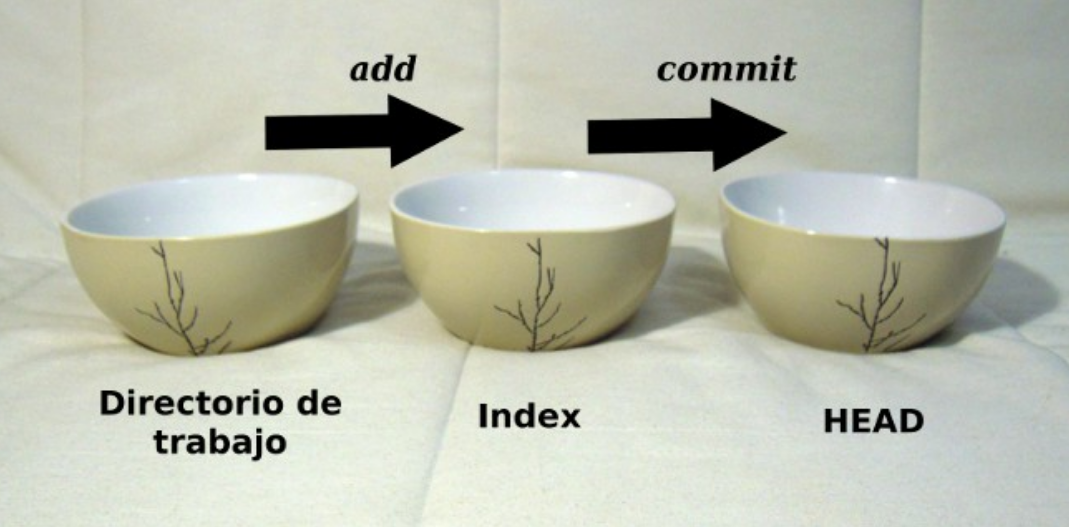
\includegraphics[width=0.8\linewidth]{img/cuencos.png}
\end{figure}
\end{frame}

\begin{frame}[fragile]
\frametitle{Cómo borrar ficheros}
Para borrar un fichero, ejecuta el siguiente comando:
\begin{block}{Comando}
\begin{verbatim}
git rm <file>
\end{verbatim}
\end{block}
\vskip 1.00cm
Para borrar un fichero del \textbf{Index}, ejecuta el siguiente comando:
\begin{block}{Comando}
\begin{verbatim}
git rm --cached <file>
\end{verbatim}
\end{block}
\end{frame}

\begin{frame}[fragile]
\frametitle{Cómo mover o renombrar ficheros}
Para mover o renombrar un fichero, ejecuta el siguiente comando:
\begin{block}{Comando}
\begin{verbatim}
git mv <file>
\end{verbatim}
\end{block}
\end{frame}

\begin{frame}[fragile]
\frametitle{Deshacer cambios en un archivo}
Para recuperar la versión del HEAD, ejecuta el siguiente comando:
\begin{block}{Comando}
\begin{verbatim}
git checkout -- <file>
\end{verbatim}
\end{block}
\end{frame}

\begin{frame}[fragile]
\frametitle{Cómo conocer el estado actual}
Para conocer el estado actual del repositorio, ejecuta el siguiente comando:
\begin{block}{Comando}
\begin{verbatim}
git status
\end{verbatim}
\end{block}
\vskip 1.00cm
Para ver las diferencias, ejecuta el siguiente comando:
\begin{block}{Comando(s)}
\begin{verbatim}
git diff
git diff <file>
\end{verbatim}
\end{block}
\end{frame}

\begin{frame}[fragile]
\frametitle{Historial}
Para mostrar el historial de todos los cambios efectuados, ejecuta el siguiente comando:
\begin{block}{Comando}
\begin{verbatim}
git log [-N]
\end{verbatim}
\end{block}
\vskip 0.50cm
Otros Parámetros:
\begin{itemize}
\item --oneline
\item --graph
\item -p
\end{itemize}
\end{frame}

\begin{frame}
\frametitle{Cómo sincronizar con un servidor remoto}
\begin{figure}
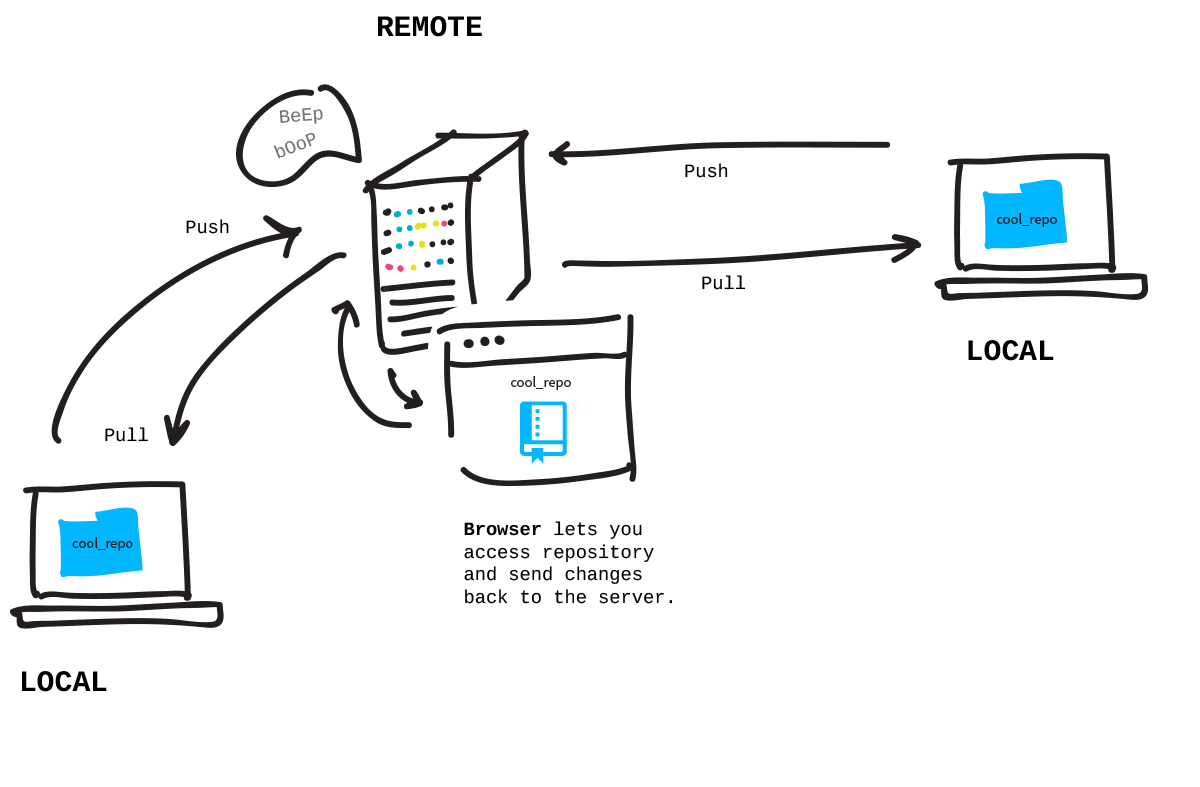
\includegraphics[width=0.95\linewidth]{img/remote.png}
\end{figure}
\end{frame}

\begin{frame}[fragile]
\frametitle{Cómo enviar los cambios al servidor remoto}
Tras registrar los cambios en el \textbf{HEAD} de la copia local, para enviar los cambios al repositorio remoto ejecuta el siguiente comando:
\begin{block}{Comando(s)}
\begin{verbatim}
git push origin master
git push
\end{verbatim}
\end{block}
\vskip 1.00cm
Si se desea registrar los cambios de otra rama, reemplaza \textit{master} por la rama deseada.
\begin{block}{Comando(s)}
\begin{verbatim}
git push origin <branch>
\end{verbatim}
\end{block}
\end{frame}

\begin{frame}[fragile]
\frametitle{Cómo actualizar el repositorio local}
Para actualizar el repositorio local, ejecuta el siguiente comando:
\begin{block}{Comando(s)}
\begin{verbatim}
git pull origin master
git pull origin <branch>
git pull
\end{verbatim}
\end{block}
\end{frame}

\begin{frame}[fragile]
\frametitle{Cómo gestionar el conflicto entre repositorios}
\begin{itemize}
\item Git informa detalladamente del problema
\item El usuario deberá arreglar el problema
\item El usuario deberá hacer \textit{commit} y \textit{push}
\end{itemize}
\end{frame}

\begin{frame}[fragile]
\frametitle{Etiquetas}
Para listar las etiquetas, ejecuta el siguiente comando:
\begin{block}{Comando}
\begin{verbatim}
git tag
\end{verbatim}
\end{block}
\vskip 0.20cm
Para crear una etiqueta, ejecuta el siguiente comando:
\begin{block}{Comando}
\begin{verbatim}
git tag v0.0.2
\end{verbatim}
\end{block}
\vskip 0.20cm
Para crear una etiqueta con una anotación, ejecuta el siguiente comando:
\begin{block}{Comando}
\begin{verbatim}
git tag -a v0.0.2 -m ``New software version.''
\end{verbatim}
\end{block}
\end{frame}

\begin{frame}[fragile]
\frametitle{Archivo .gitignore}
A menudo, hay archivos que no se desean que sean añadidos al repositorio: passwords, temporales, binarios compilados, archivos de configuración local, etc.
\begin{itemize}
\item Git permite utilizar archivos en los que se indica qué archivos debe ignorar
\item Archivo: \textbf{.gitignore}
\item Uso de expresiones regulares y comentarios
\end{itemize}
\vskip 0.50cm
\begin{block}{Ejemplo}
\begin{verbatim}
# Byte-compiled / optimized / DLL files
__pycache__/
*.py[cod]
\end{verbatim}
\end{block}
\end{frame}

\begin{frame}[fragile]
\frametitle{Ramas}
Para crear una nueva rama, ejecuta el siguiente comando:
\begin{block}{Comando}
\begin{verbatim}
git branch <new-branch-name>
\end{verbatim}
\end{block}
\vskip 0.25cm
Para moverse a la rama creada, ejecuta el siguiente comando:
\begin{block}{Comando}
\begin{verbatim}
git checkout <new-branch-name>
\end{verbatim}
\end{block}
\vskip 0.25cm
Para volver a la rama principal, ejecuta el siguiente comando:
\begin{block}{Comando}
\begin{verbatim}
git checkout master
\end{verbatim}
\end{block}
\end{frame}

\begin{frame}[fragile]
\frametitle{Ramas}
Para borrar una rama, ejecuta el siguiente comando:
\begin{block}{Comando}
\begin{verbatim}
git branch -d <new-branch-name>
\end{verbatim}
\end{block}
\vskip 0.50cm
Para enviar una rama al repositorio remoto, ejecuta el siguiente comando:
\begin{block}{Comando}
\begin{verbatim}
git push origin <new-branch-name>
\end{verbatim}
\end{block}
\end{frame}

\begin{frame}[fragile]
\frametitle{Ramas}
Para fusionar una rama a la rama activa, ejecuta el siguiente comando:
\begin{block}{Comando}
\begin{verbatim}
git merge <new-branch-name>
\end{verbatim}
\end{block}
\vskip 0.50cm
Antes de ejecutar ese comando se recomienda comparar los cambios. Para ello, ejecuta el siguiente comando:
\begin{block}{Comando}
\begin{verbatim}
git diff <source-branch> <target-branch>
\end{verbatim}
\end{block}
\end{frame}

\begin{frame}
\frametitle{Ramas: Manejo básico}
\begin{figure}
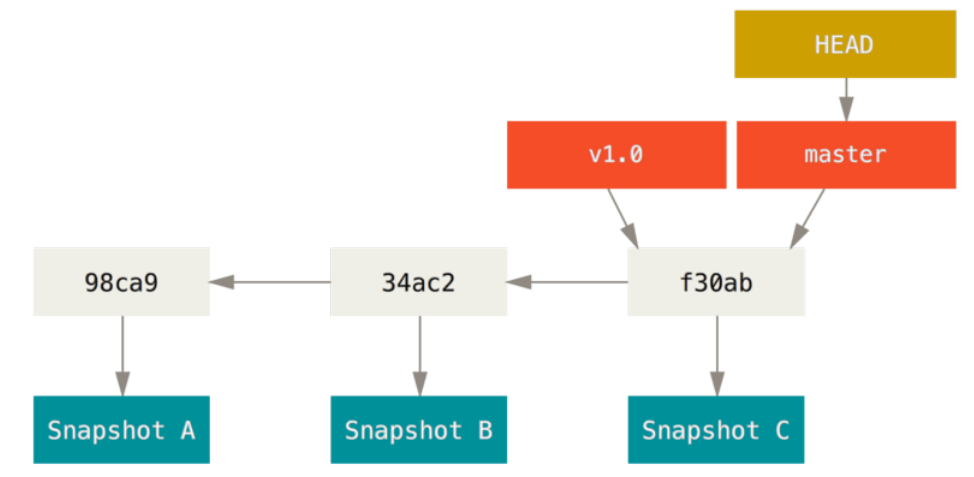
\includegraphics[width=0.85\linewidth]{img/branching-0.png}
\end{figure}
\end{frame}

\begin{frame}
\frametitle{Ramas: Manejo básico}
\begin{figure}
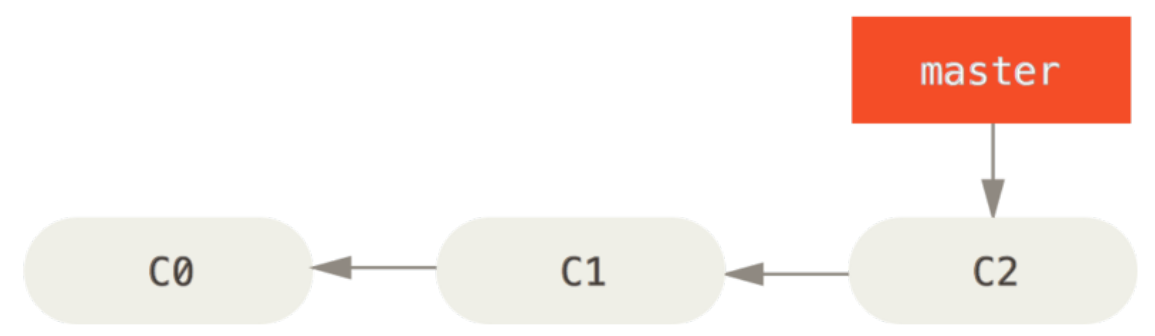
\includegraphics[width=0.85\linewidth]{img/branching-1.png}
\end{figure}
\end{frame}

\begin{frame}[fragile]
\frametitle{Ramas: Manejo básico}
\begin{figure}
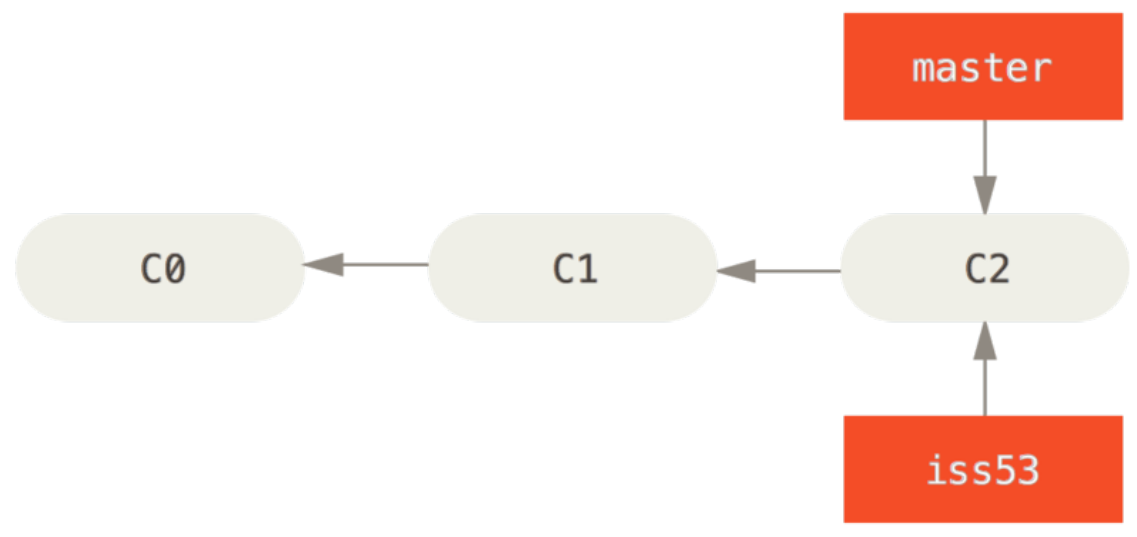
\includegraphics[width=0.85\linewidth]{img/branching-2.png}
\end{figure}
\vskip 0.50cm
\footnotesize
\begin{block}{Comando(s)}
\begin{verbatim}
git branch iss53
git checkout iss53
\end{verbatim}
\end{block}
\end{frame}

\begin{frame}[fragile]
\frametitle{Ramas: Manejo básico}
\begin{figure}
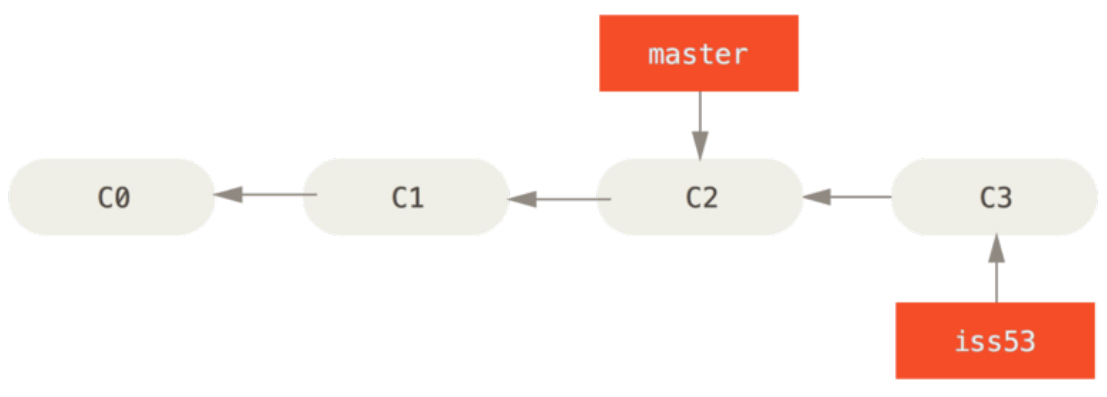
\includegraphics[width=0.85\linewidth]{img/branching-3.png}
\end{figure}
\vskip 0.50cm
\footnotesize
\begin{block}{Comando(s)}
\begin{verbatim}
vim index.html
git commit -a -m 'added a new footer [issue 53]'
\end{verbatim}
\end{block}
\end{frame}

\begin{frame}[fragile]
\frametitle{Ramas: Manejo básico}
\begin{figure}
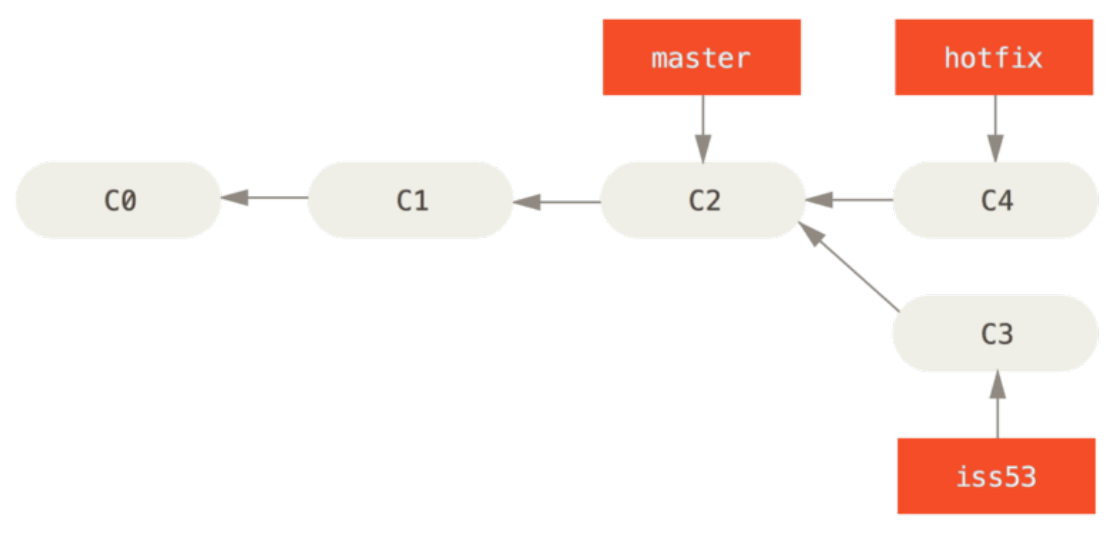
\includegraphics[width=0.70\linewidth]{img/branching-4.png}
\end{figure}
\vskip 0.10cm
\scriptsize
\begin{block}{Comando(s)}
\begin{verbatim}
git checkout master
git branch hotfix
git checkout hotfix
vim index.html
git commit -a -m 'fixed the broken email address'
\end{verbatim}
\end{block}
\end{frame}

\begin{frame}[fragile]
\frametitle{Ramas: Manejo básico}
\begin{figure}
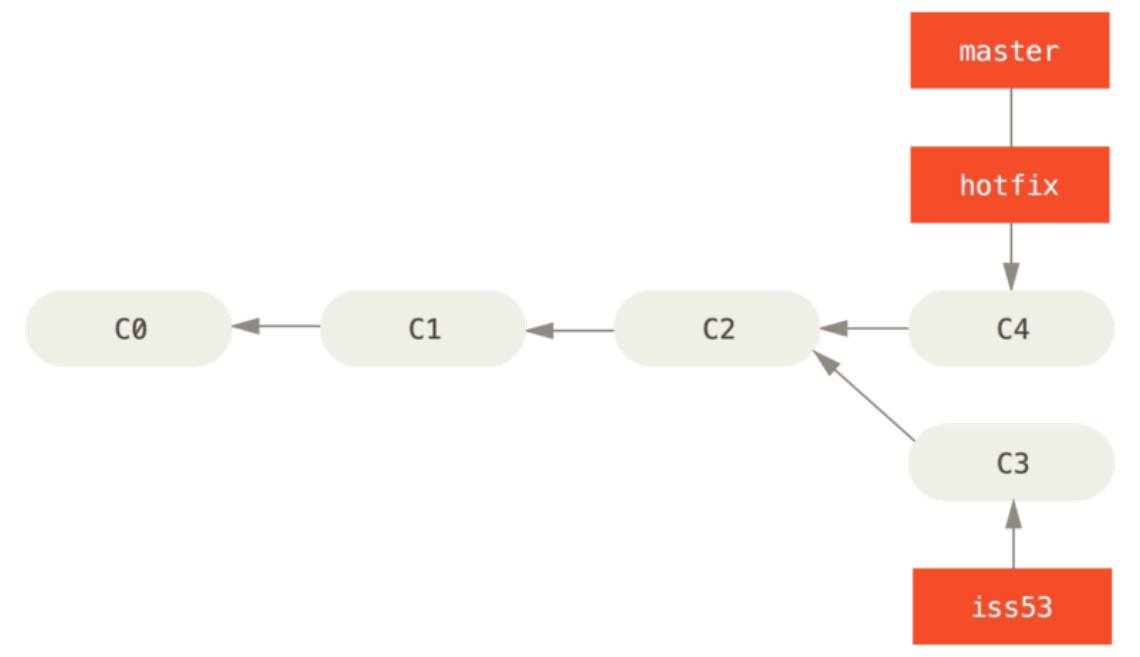
\includegraphics[width=0.70\linewidth]{img/branching-5.png}
\end{figure}
\vskip 0.30cm
\footnotesize
\begin{block}{Comando(s)}
\begin{verbatim}
git checkout master
git merge hotfix
\end{verbatim}
\end{block}
\end{frame}

\begin{frame}[fragile]
\frametitle{Ramas: Manejo básico}
\begin{figure}
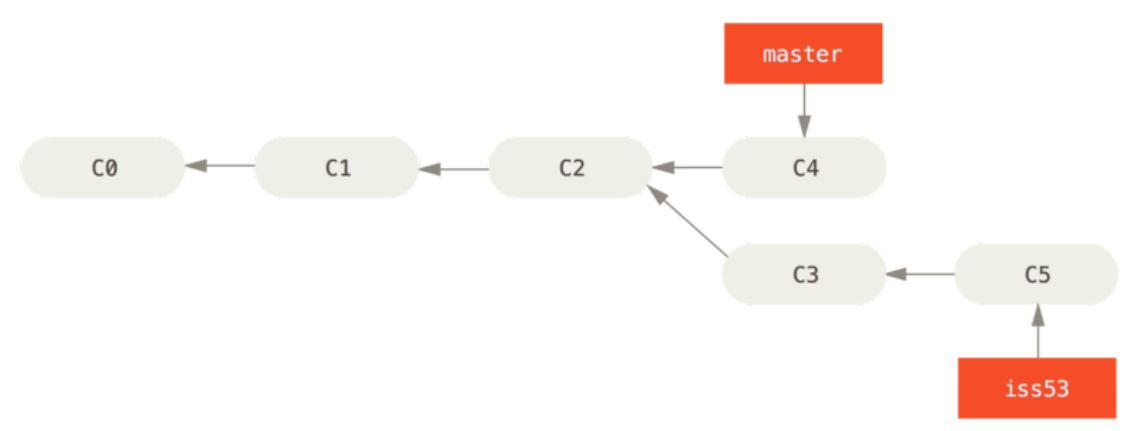
\includegraphics[width=0.85\linewidth]{img/branching-6.png}
\end{figure}
\vskip 0.30cm
\footnotesize
\begin{block}{Comando(s)}
\begin{verbatim}
git branch -d hotfix
---
git checkout iss53
vim index.html
git commit -a -m 'finished the new footer [issue 53]'
\end{verbatim}
\end{block}
\end{frame}

\begin{frame}[fragile]
\frametitle{Ramas: Manejo básico}
\begin{figure}
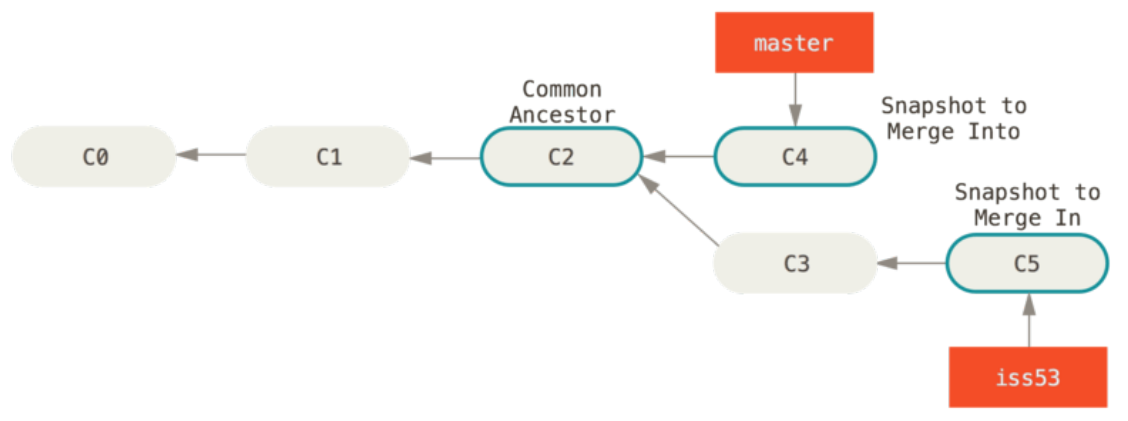
\includegraphics[width=0.85\linewidth]{img/branching-7.png}
\end{figure}
\vskip 0.30cm
\footnotesize
\begin{block}{Comando(s)}
\begin{verbatim}
git checkout master
git merge iss53
\end{verbatim}
\end{block}
\end{frame}

\begin{frame}[fragile]
\frametitle{Ramas: Manejo básico}
\begin{figure}
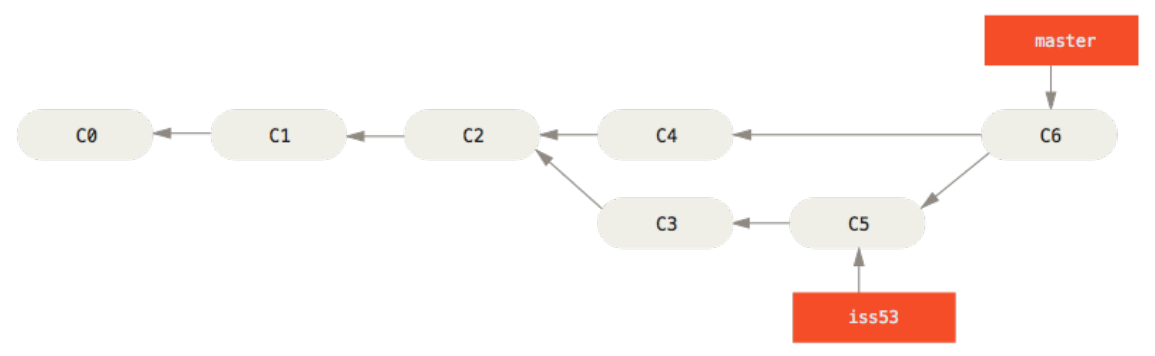
\includegraphics[width=0.85\linewidth]{img/branching-8.png}
\end{figure}
\vskip 0.30cm
\footnotesize
\begin{block}{Comando(s)}
\begin{verbatim}
git checkout master
git merge iss53
\end{verbatim}
\end{block}
\end{frame}

\begin{frame}
\frametitle{Ramas: Flujo de trabajo}
\begin{figure}
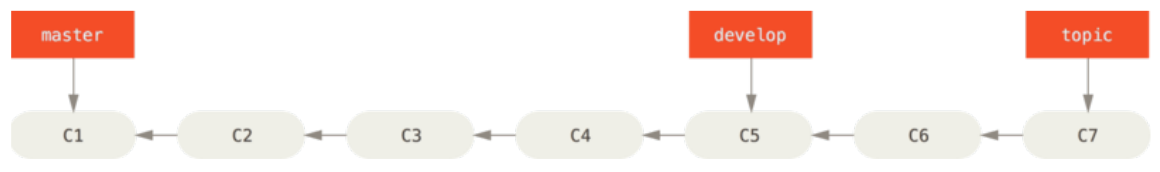
\includegraphics[width=0.90\linewidth]{img/branching-9.png}
\end{figure}
\begin{figure}
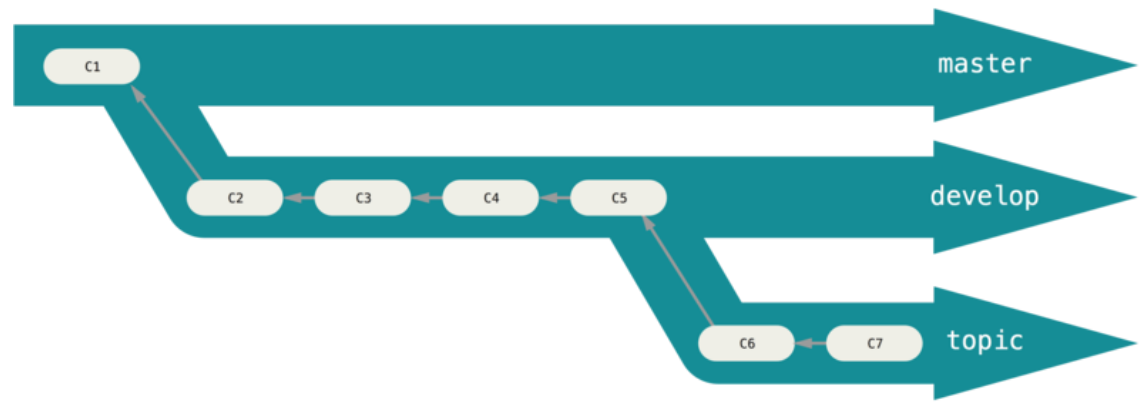
\includegraphics[width=0.90\linewidth]{img/branching-10.png}
\end{figure}
\end{frame}

\begin{frame}
\frametitle{Referencias}
\begin{thebibliography}{99}
\tiny
\bibitem{} Scott Chacon y Ben Straub
\newblock Pro Git
\newblock https://git-scm.com/book/en/v2
\bibitem{} Pablo Hinojosa y JJ Merelo
\newblock Aprende git
\newblock https://github.com/JJ/aprende-git
\bibitem{} Angel Pablo Hinojosa Gutiérrez
\newblock El Zen de git
\newblock http://www.psicobyte.com/descargas/ZenDeGit.pdf
\newblock https://www.youtube.com/watch?v=P4RcOZycZBM
\bibitem{} Mark Lodato
\newblock A Visual Git Reference
\newblock http://marklodato.github.io/visual-git-guide/index-en.html
\bibitem{} Roger Dudler 
\newblock Git - la guía sencilla
\newblock http://rogerdudler.github.io/git-guide/index.es.html
\bibitem{} Víctor Suárez García
\newblock  Introducción a Git
\newblock http://slides.com/zerasul/git/
\bibitem{} Rafael Rodriguez
\newblock My Work From FreeCodeCamp
\newblock https://github.com/Rafase282/My-FreeCodeCamp-Code
\end{thebibliography}
\end{frame}

\begin{frame}
\Huge{\centerline{¡Muchas gracias!}}
\vskip 1.50cm
\small{\centerline{Rubén Crespo Cano}}
\vskip 0.15cm
\small{\centerline{{\color{gray}\textit{@rcrespocano}}}}
\end{frame}

\end{document}
